\documentclass{ximera}

\graphicspath{  
{./}
{./whoAreYou/}
{./drawingWithTheTurtle/}
{./bisectionMethod/}
{./circles/}
{./anglesAndRightTriangles/}
{./lawOfSines/}
{./lawOfCosines/}
{./plotter/}
{./staircases/}
{./pitch/}
{./qualityControl/}
{./symmetry/}
{./nGonBlock/}
}


%% page layout
\usepackage[cm,headings]{fullpage}
\raggedright
\setlength\headheight{13.6pt}


%% fonts
\usepackage{euler}

\usepackage{FiraMono}
\renewcommand\familydefault{\ttdefault} 
\usepackage[defaultmathsizes]{mathastext}
\usepackage[htt]{hyphenat}

\usepackage[T1]{fontenc}
\usepackage[scaled=1]{FiraSans}

%\usepackage{wedn}
\usepackage{pbsi} %% Answer font


\usepackage{cancel} %% strike through in pitch/pitch.tex


%% \usepackage{ulem} %% 
%% \renewcommand{\ULthickness}{2pt}% changes underline thickness

\tikzset{>=stealth}

\usepackage{adjustbox}

\setcounter{titlenumber}{-1}

%% journal style
\makeatletter
\newcommand\journalstyle{%
  \def\activitystyle{activity-chapter}
  \def\maketitle{%
    \addtocounter{titlenumber}{1}%
                {\flushleft\small\sffamily\bfseries\@pretitle\par\vspace{-1.5em}}%
                {\flushleft\LARGE\sffamily\bfseries\thetitlenumber\hspace{1em}\@title \par }%
                {\vskip .6em\noindent\textit\theabstract\setcounter{question}{0}\setcounter{sectiontitlenumber}{0}}%
                    \par\vspace{2em}
                    \phantomsection\addcontentsline{toc}{section}{\thetitlenumber\hspace{1em}\textbf{\@title}}%
                     }}
\makeatother



%% thm like environments
\let\question\relax
\let\endquestion\relax

\newtheoremstyle{QuestionStyle}{\topsep}{\topsep}%%% space between body and thm
		{}                      %%% Thm body font
		{}                              %%% Indent amount (empty = no indent)
		{\bfseries}            %%% Thm head font
		{)}                              %%% Punctuation after thm head
		{ }                           %%% Space after thm head
		{\thmnumber{#2}\thmnote{ \bfseries(#3)}}%%% Thm head spec
\theoremstyle{QuestionStyle}
\newtheorem{question}{}



\let\freeResponse\relax
\let\endfreeResponse\relax

%% \newtheoremstyle{ResponseStyle}{\topsep}{\topsep}%%% space between body and thm
%% 		{\wedn\bfseries}                      %%% Thm body font
%% 		{}                              %%% Indent amount (empty = no indent)
%% 		{\wedn\bfseries}            %%% Thm head font
%% 		{}                              %%% Punctuation after thm head
%% 		{3ex}                           %%% Space after thm head
%% 		{\underline{\underline{\thmname{#1}}}}%%% Thm head spec
%% \theoremstyle{ResponseStyle}

\usepackage[tikz]{mdframed}
\mdfdefinestyle{ResponseStyle}{leftmargin=1cm,linecolor=black,roundcorner=5pt,
, font=\bsifamily,}%font=\wedn\bfseries\upshape,}


\ifhandout
\NewEnviron{freeResponse}{}
\else
%\newtheorem{freeResponse}{Response:}
\newenvironment{freeResponse}{\begin{mdframed}[style=ResponseStyle]}{\end{mdframed}}
\fi



%% attempting to automate outcomes.

%% \newwrite\outcomefile
%%   \immediate\openout\outcomefile=\jobname.oc
%% \renewcommand{\outcome}[1]{\edef\theoutcomes{\theoutcomes #1~}%
%% \immediate\write\outcomefile{\unexpanded{\outcome}{#1}}}

%% \newcommand{\outcomelist}{\begin{itemize}\theoutcomes\end{itemize}}

%% \NewEnviron{listOutcomes}{\small\sffamily
%% After answering the following questions, students should be able to:
%% \begin{itemize}
%% \BODY
%% \end{itemize}
%% }
\usepackage[tikz]{mdframed}
\mdfdefinestyle{OutcomeStyle}{leftmargin=2cm,rightmargin=2cm,linecolor=black,roundcorner=5pt,
, font=\small\sffamily,}%font=\wedn\bfseries\upshape,}
\newenvironment{listOutcomes}{\begin{mdframed}[style=OutcomeStyle]After answering the following questions, students should be able to:\begin{itemize}}{\end{itemize}\end{mdframed}}



%% my commands

\newcommand{\snap}{{\bfseries\itshape\textsf{Snap!}}}
\newcommand{\flavor}{\link[\snap]{https://snap.berkeley.edu/}}
\newcommand{\mooculus}{\textsf{\textbf{MOOC}\textnormal{\textsf{ULUS}}}}


\usepackage{tkz-euclide}
\tikzstyle geometryDiagrams=[rounded corners=.5pt,ultra thick,color=black]
\colorlet{penColor}{black} % Color of a curve in a plot



\ifhandout\newcommand{\mynewpage}{\newpage}\else\newcommand{\mynewpage}{}\fi



\title{Similar triangles}

\author{Bart Snapp}



\begin{document}
\begin{abstract}
  We talk about similar triangles.
\end{abstract}
\maketitle

In geometry, we may have several different segments all with the same
length. We don't want to say that the segments are \textit{equal}
because that would mean that they are \textit{exactly} the
same---position included. Hence we need a new concept:

\begin{definition}\index{congruent!segments}
When different segments have the same length, we say they are
\textbf{congruent segments}. 
\end{definition}

\begin{definition}\index{congruent!angles}
In a similar fashion, if there is an isometry that maps one angle to another angle, then we say they are \textbf{congruent angles}.
\end{definition}

Putting these together, we have the definition for triangles:

\begin{definition}\index{congruent!triangles} 
Two triangles are said to be \textbf{congruent triangles} if there is
an isometry that maps one triangle to the other triangle.
\end{definition}


After working with triangles for short time, one quickly sees that the
notion of congruence is not the only ``equivalence'' one wants to
make between triangles. In particular, we want the notion of
\textit{similarity.} \index{similar triangles}

One day when aloof old Professor Rufus was trying to explain similar
triangles to his class, he merely wrote
\[
\tri ABC \sim \tri A'B'C' \qquad\Leftrightarrow \qquad\begin{array}{l}
\angle A \simeq \angle A'\\
\angle B \simeq \angle B' \\
\angle C \simeq \angle C'
\end{array}
\]
and walked out of the room.

\begin{question} 
Can you give three much needed examples of similar triangles? 
\end{question}


%% \begin{question} 
%% Devise a way to use folding and tracing constructions to help explore this notion
%% of similar triangles.
%% \end{question}


Another day when aloof old Professor Rufus was trying to explain
similar triangles to his class, he merely wrote
\[
\tri ABC \sim \tri A'B'C' \qquad\Leftrightarrow \qquad
\begin{array}{l}
AB = k\cdot A'B'\\
BC = k\cdot B'C' \\
CA = k\cdot C'A'
\end{array}
\]
and walked out of the room.

\begin{question} 
Can you give three much needed examples of similar triangles? 
\end{question}


\begin{question} 
Devise a way to use folding and tracing constructions to help explore this notion
of similar triangles.
\end{question}




\begin{question} 
What's going on in aloof old Professor Rufus' head\footnote{I realize that
this is a dangerous question!}---why are his explanations so different?
\end{question}


In fact, the two definitions of similar triangles given
above are \textbf{equivalent}.


\begin{definition}\index{similar triangles} 
Two triangles $\tri ABC$ and $\tri A'B'C'$ are said to be
\textbf{similar} if either equivalent condition holds:
\[
\begin{array}{l}
\angle A \simeq \angle A'\\
\angle B \simeq \angle B' \\
\angle C \simeq \angle C'
\end{array}
\qquad\text{or}\qquad
\begin{array}{l}
AB = k\cdot A'B'\\
BC = k\cdot B'C' \\
CA = k\cdot C'A'
\end{array}
\]
\end{definition}

Let's see if we can put similar triangles to work. Here is an old
carpenter's trick. Suppose you have two parallel lines.  
\[

\includegraphics{twoLinesCarp.pdf}
\]
If you want to make two more lines that divide the space into three
equal regions, you can place a ruler diagonally across the parallel
lines, and then mark off one-third of the diagonal distance. 
\[
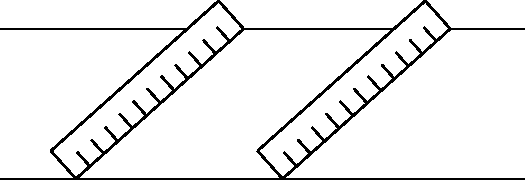
\includegraphics{twoLinesCarpRulers.pdf}
\]
From this you get your three regions.
\[
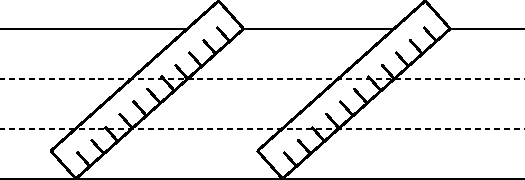
\includegraphics{twoLinesCarpRulersLines.pdf}
\]
\begin{question}
Can you explain why this works using similar triangles?
\end{question}


Now for a more challenging situation.  Suppose we have an equilateral
triangle of side length $2$. Use similar triangles and the Pythagorean
Theorem to find the length of the segment $a$ (the segment that goes
from the \textbf{center} of the triangle to a side at a right angle)
in the picture below.
\[
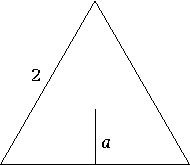
\includegraphics{triangleSegment.pdf}
\]
\begin{question}
How do you do this?
\end{question}


\end{document}
